% document settings
%%%%%%%%%%%%%%%%%%%%%%%%%%%%%%%%%%%%
\documentclass[final,5p,times,twocolumn,11pt]{elsarticle}


% standard packages
%%%%%%%%%%%%%%%%%%%%%%%%%%%%%%%%%%%%
\usepackage{graphicx}
\usepackage{amssymb}
\usepackage{amsmath}
\usepackage{empheq} 
\usepackage{comment}
\usepackage{enumerate}
\usepackage{setspace}
\usepackage[inline,shortlabels]{enumitem}


% other packages 
%%%%%%%%%%%%%%%%%%%%%%%%%%%%%%%%%%%%
\usepackage{balance} 					% to balance the last columns 
\usepackage[usenames,dvipsnames]{color} 	% to get color with fancy colornames
\usepackage{floatpag} 					% remove page number for figure that covers entire page
\usepackage{bbm}						% for indicator function with \mathbbm{1}
\usepackage[normalem]{ulem} 				% for tables
\useunder{\uline}{\ul}{} 					% for tables



% some settings
%%%%%%%%%%%%%%%%%%%%%%%%%%%%%%%%%%%%
\numberwithin{equation}{section} % numerates equations according to sections	
\linespread{1.2} 		           % space between lines

 % bibilography settings
%%%%%%%%%%%%%%%%%%%%%%%%%%%%%%%%%%%%%%%%%%%%%%%%%%%%%%%%%%%%%%%%%%%%%%%%%%%%%%
\biboptions{sort&compress} % cite as [1,2,3] and not [3,1,2] etc. 	

% bug fix in elsearticle
%%%%%%%%%%%%%%%%%%%%%%%%%%%%%%%%%%%%
\makeatletter
\def\@author#1{\g@addto@macro\elsauthors{\normalsize%
    \def\baselinestretch{1}%
    \upshape\authorsep#1\unskip\textsuperscript{%
      \ifx\@fnmark\@empty\else\unskip\sep\@fnmark\let\sep=,\fi
      \ifx\@corref\@empty\else\unskip\sep\@corref\let\sep=,\fi
      }%
    \def\authorsep{\unskip,\space}%
    \global\let\@fnmark\@empty
    \global\let\@corref\@empty  %% Added
    \global\let\sep\@empty}%
    \@eadauthor={#1}
}
\makeatother


% This removes the Preprint `submitted to "Journal_name"' footnote.
%%%%%%%%%%%%%%%%%%%%%%%%%%%%%%%%%%%%
\makeatletter
\def\ps@pprintTitle{%
 \let\@oddhead\@empty 
 \let\@evenhead\@empty
 \def\@oddfoot{}%
 \let\@evenfoot\@oddfoot}
 \makeatother
 
 
 % specify the colors of links
 %%%%%%%%%%%%%%%%%%%%%%%%%%%%%%%%%%%%
\usepackage[table,xcdraw,svgnames]{xcolor}
\usepackage[colorlinks]{hyperref}
\AtBeginDocument{%
  \hypersetup{
    citecolor=SteelBlue,
    linkcolor=SteelBlue,   
    urlcolor=SteelBlue}
   }
   
  % shortcuts & makros
%%%%%%%%%%%%%%%%%%%%%%%%%%%%%%%%%%%%%%%%%%%%%%%%%%%%%%%%%%%%%%%%%%
\newcommand{\red}[1]{\textcolor{WildStrawberry}{#1}} 					%  red text
\newcommand{\pd}[2]{ \frac{\partial #1}{\partial #2}} 						% first partial derivative
\newcommand{\pdt}[2]{\frac{\partial^2 #1}{\partial #2^2}} 					% second partial derivative 
\newcommand{\td}[2]{ \frac{\mathrm{d} #1}{\mathrm{d} #2}}				 % first total derivative
\newcommand{\tdt}[2]{ \frac{\mathrm{d}^2 #1}{\mathrm{d} #2^2}}			 % second total derivative
\newcommand{\nt}[3]{\int \limits_{#1}^{#2} \mathrm{d}#3~} 				% integral with boundaries
\newcommand{\dd}{\mathrm{d}} 									% differential d
\newcommand{\ord}[1]{\mathcal{O} \left( #1 \right)} 						% Landau
\newcommand{\mw}[1]{\left< #1 \right>} 								% mean value
\newcommand{\expt}[2]{\mathbb{E}_{#2} \left[ #1 \right]}					% expectation value
\newcommand{\exptn}[3]{\mathbb{E}_{#2}^{(#3)} \left[ #1 \right]}			% n-th order expectation value
\newcommand{\exptc}[3]{\mathbb{E}_{#2} \left[ #1 ~ \left|  #3 \right. \right]} 	% conditional expectation value
 

% title, authors and affiliations
%%%%%%%%%%%%%%%%%%%%%%%%%%%%%%%%%%%%
\journal{~}
\begin{document}
\begin{frontmatter}

\title{Why a digital tax may be the only sustainable solution}

\author[add1]{Nate Dwyer}
\ead{nate9799@gmail.com}

\author[add1]{Sandro Claudio Lera}
\ead{slera@mit.edu}

\author[add1]{Alex `Sandy' Pentland}
\ead{sandy@media.mit.edu}

\address[add1]{\scriptsize Massachusetts Institute of Technology, 77 Massachusetts Avenue, 02139 Cambridge, Massachusetts, USA}

%%%%%%%%%%%%%%%%%%%%%%%%%%%%%%%%%%%%
\end{frontmatter}
%%%%%%%%%%%%%%%%%%%%%%%%%%%%%%%%%%%%


\section{Introduction}
\label{sec:Introduction}
%%%%%%%%%%%%%%%%%%%%%%%%%%%%%%%%%%%%%%%%%%%%%%%%%%%%%%%%%%%%%%%% 
Over time, new innovations have drastically lowered the cost of transactions.
This has had many positive effects, including increasing trade and wealth while
reducing inequities between cities and rural areas. Unfortunately,
as the transaction costs get very close to 0, monopolization and centralization
of firms becomes more likely and more profitable. This holds especially true
with technology companies, who have very low transaction costs, and are easy to
scale up. Recently, France imposed a  digital tax of 3\% [details here]. The
new French tax could serve as part of a strategy to prevent firms becoming
monopoly powers.

To see what impact extremely low transaction costs could have, we developed a
model that puts a cost on transactions proportional to the distance between a
buyer-seller pair. In this model, sellers can choose different prices and
different capacities, which allows us to model sellers modifying prices and
capacities to compensate for differing transaction costs. For example, a seller
trying to grab a larger market share might lower their prices, while a seller
close to a lot of buyers might want to produce more than a seller that is only
near a few.

\section{Model Definition}
%%%%%%%%%%%%%%%%%%%%%%%%%%%%%%%%%%%%%%%%%%%%%%%%%%%%%%%%%%%%%%%%%%%%%%%%%%%%

Our model of buyers and sellers takes place on some world with a distance
metric (e.g. a country using road distance) and studies how sellers respond to
reductions in distance based transaction costs.

To model distance based transaction costs, we need a concept of distance.  In
the real world, we could use physical distance, but in our model, we place the
buyers and sellers on a circle of circumference 1 and use the arc distance.
We then use that distance as the basis for the transaction cost, treating it as
if it were a percentage tax. More specifically, the transaction cost $t$ for
buyer $b$ to buy from seller $s$ is $p_s * \lambda d(b, s)$, where $p_s$ is the
price $s$ offers, $d(b, s)$ is the distance between buyer $b$ and seller $s$,
and $\lambda$ is a scaling factor. Lowering $\lambda$ is how we model
decreasing transaction costs.

Each buyer has an individual, linear demand curve that is negatively sloped,
meaning that the more expensive the product, the less the buyer purchases.
Buyers also always buy the from the cheapest available seller.

To separate fit sellers from unfit sellers, we use assign sellers differing
cost-per-unit values, with more competitive sellers having lower cost-per-unit
values than less competitive sellers.

@Sandro: Should I even include the math parts?

On the circle, the sellers will play a two step game (known as a
Kreps-Schienkman game) where each seller $s$ will first determine and announce
their capacity $\hat q_s$ (the maximum amount of product they can sell), then
determine and announce their price $p_s$. They choose their capacity and price
trying to maximize their profit $$\Pi = p_sq_s - c_s\hat q_s,$$ where $q_s$ is
the quantity the seller actually sells, and $c_s$ is the cost-per-unit. 

\section{Results}
We can see in Figure \ref{fig:no_tax}, where $\lambda=0$ and there is no
transaction cost, that Firm 1 is able to make 33\% more profit despite only a
1\% lower cost-per-unit. But in Figure \ref{fig:no_tax}, where there is a
significant transaction cost of $\lambda = .4$, the difference in profits
is much closer, with Firm 1 only earning 8\% more than firm 2, with the same
1\% difference in costs. This decrease in monopolization comes at a great cost
though, as both firm's profit in the first scenario is significantly higher
than in the second.

\begin{figure}[!htb]
	\centering
	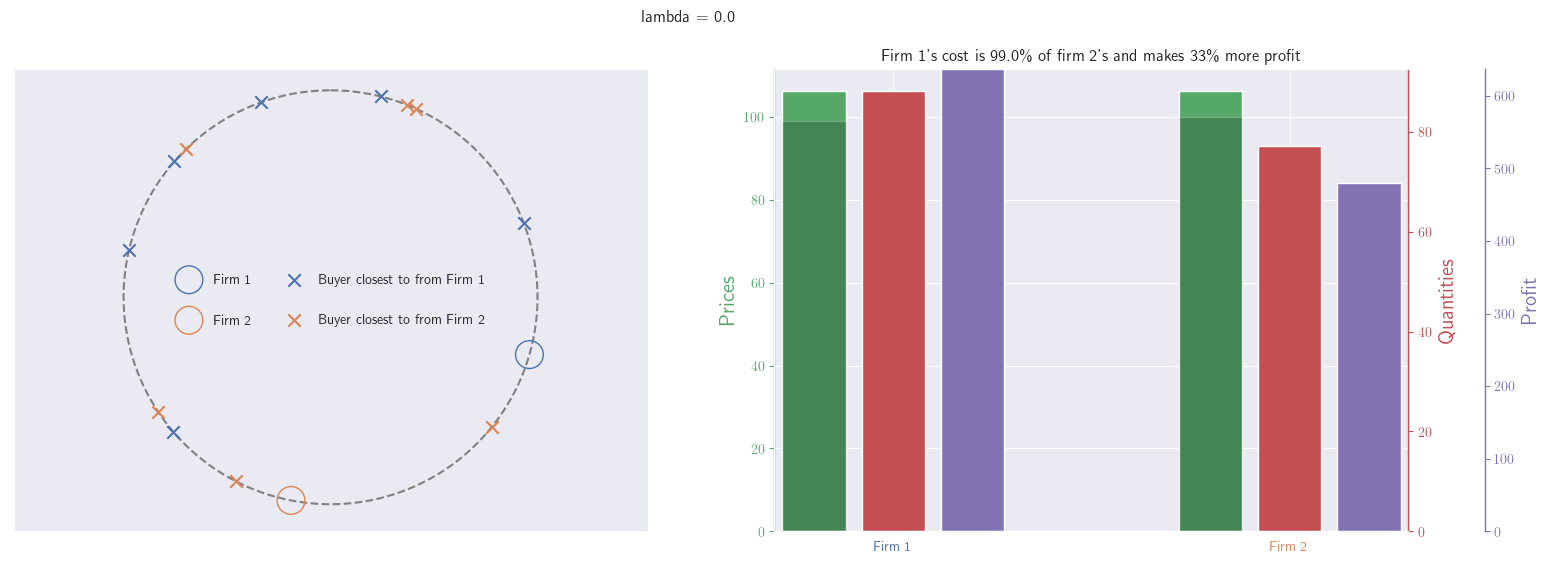
\includegraphics[width=\textwidth/2]{no_tax.png}
	\caption{The trade-offs of the transaction costs are demonstrated.
		This figure depicts an economy where the is no distance-based tax. In the economy, the profits of both firms are high, but one firm has 33\% larger profits because of a slight advantage in having 1\% cheaper unit costs.}
	\label{fig:no_tax}
\end{figure}

\begin{figure}[!htb]
	\centering
	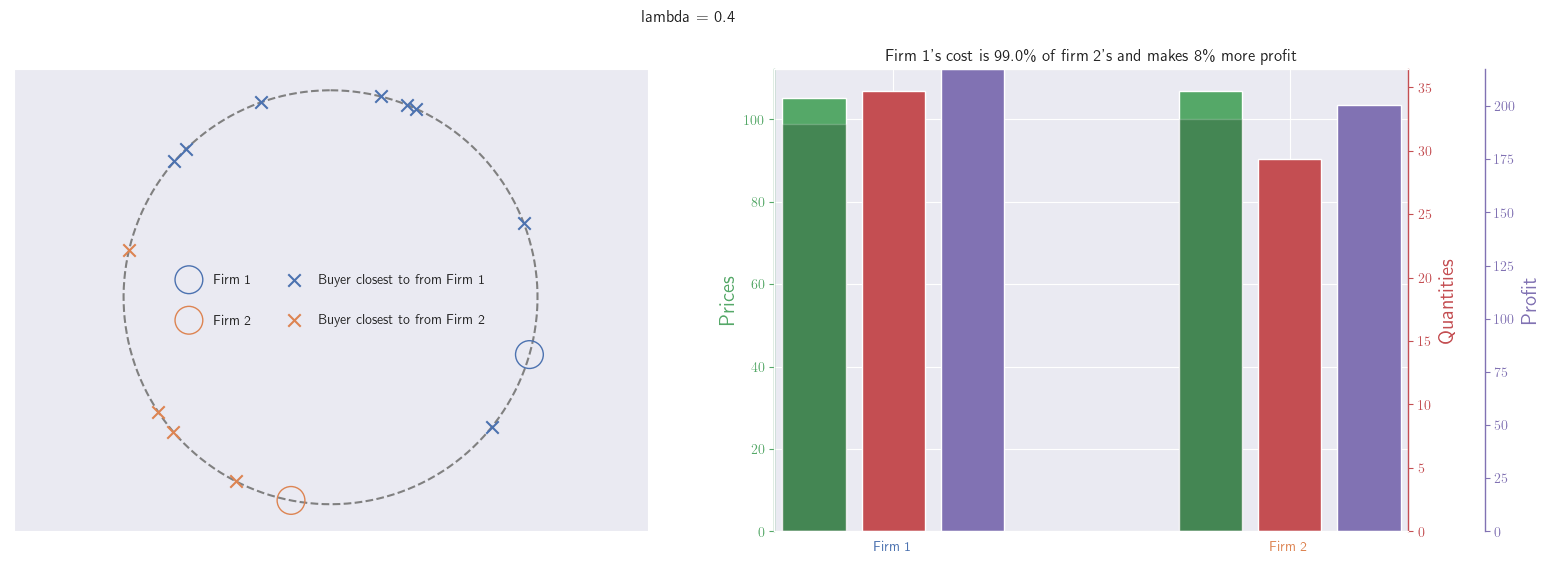
\includegraphics[width=\textwidth/2]{lambda=4Over10.png}
	\caption{
		In contrast to Figure \ref{fig:no_tax}, this figure depicts an economy with a significant transaction cost. The profits for both firms are significantly lower, but also are much closer, with Firm 1 earning 8\% more profit, as opposed to 33\% in the previous figure.}
	\label{fig:lambda=.4}
\end{figure}

\section{Iterating the Model}
This difference becomes even more apparent when we iterate the model and
include a feedback mechanism. In such a game, a small initial advantage could
lead to rapid monopolization when there is no friction in the market, such as
transaction costs. However, in a market with some, small transaction costs, the
two firms can stay competitive and neither firm will become the monopoly power.

\section{Conclusion}

At MIT, we are currently developing a new form of taxation that leverages
benefits of digital market place with this mechanism. We hope to still capture
all of the benefits of low transaction costs, including increased trade,
profit, and  fairness, while at the same time reducing the ability and
incentive for sellers to monopolize.

\section{Side Notes}
Since we are now using a physical distance instead of an ordinal distance, when $\lambda$ is high, the transaction cost can be more important than the cost-per-unit in determining profit and relative fitness of firms.

In addition, our model may not be an accurate descriptor of how a tech company works, as it would seem more accurate for tech companies to have a very low or no per-unit-costs, instead having high fixed costs.

\end{document}